\subsection{Manuscript Management}

\subsubsection{Scope}
\par{This section provides the detailed service contracts and activity diagrams(where needed) for the use cases offered by the Manuscript Management module.
It's services includes all the needed functionality to create, read, evaluate, edit and to send it to the next role in the life-cycle of creating a quality book.}

\begin{figure}[h]
	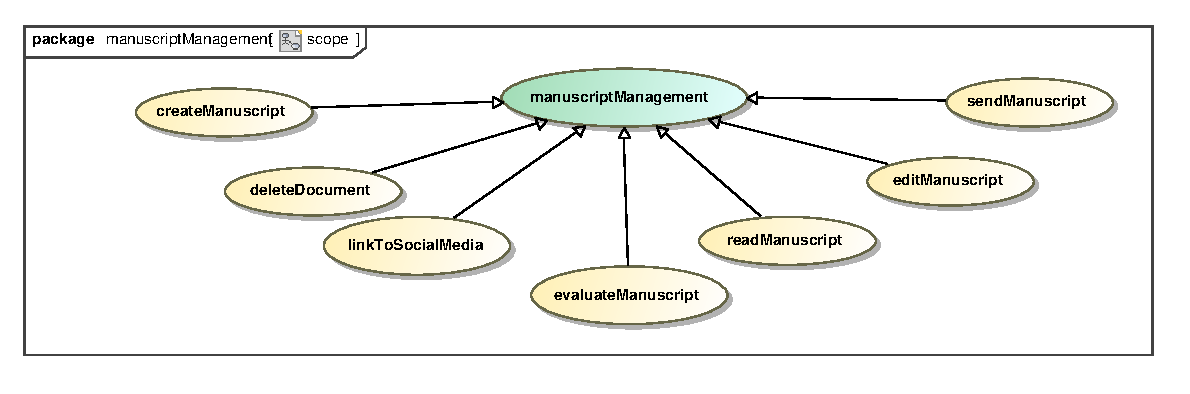
\includegraphics[height=200px, width=500px]{epsImages/ManuscriptManagement/scope.eps}
	\caption{Scope for manuscript management module}
\end{figure}

\newpage
\subsubsection{Use Cases}
\begin{enumerate}
\item \textbf{Create Manuscript - priority: critical}

\par{This use case allows an author to create a new project, by creating a new manuscript. The author will be able to give the manuscript a name(title) and specify the privacy setting on it. There may be one or multiple authors collaborating on a manuscript.
A manuscript's title should be unique.}\\

\textbf{Service Contract:}

\begin{figure}[h]
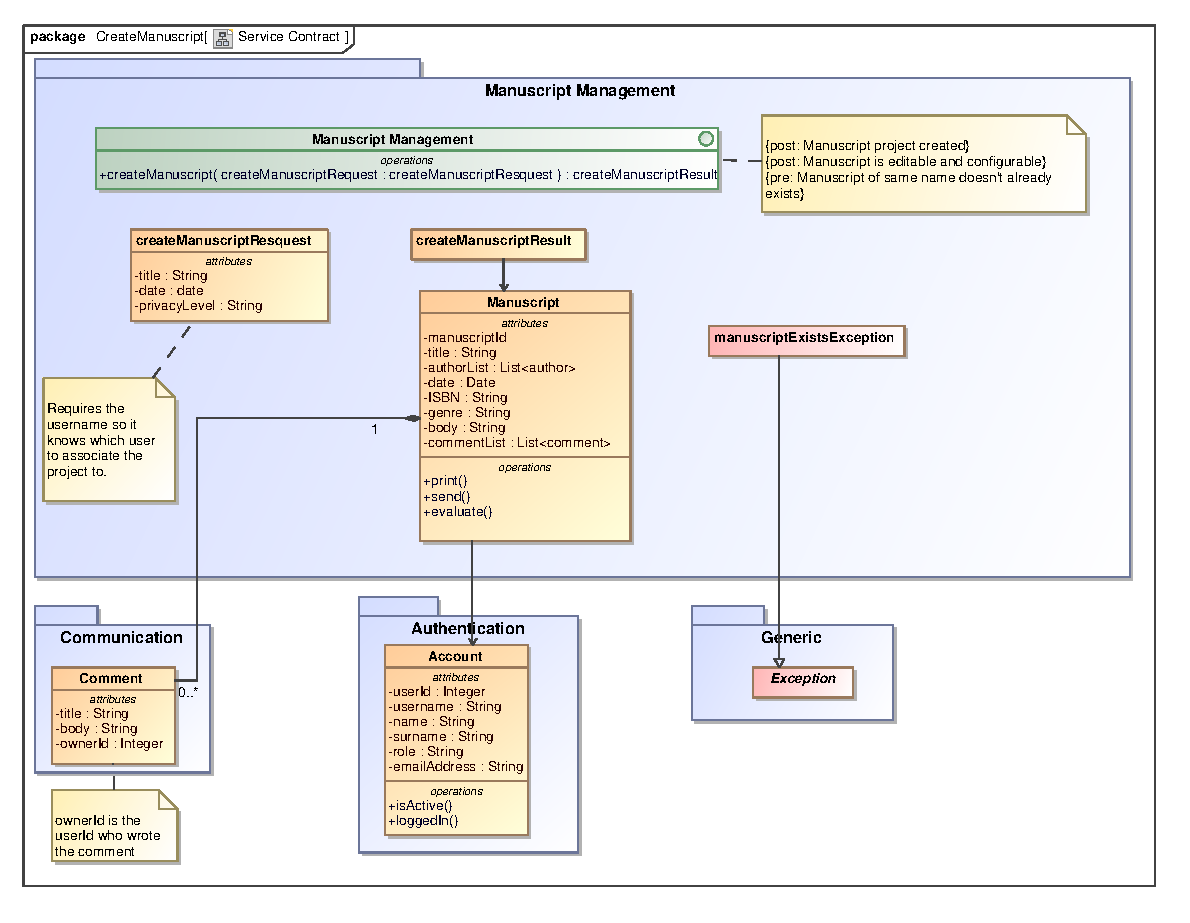
\includegraphics[height=330px, width=500px]{epsImages/ManuscriptManagement/createManuscriptServiceContract.eps}
\caption{Service contract for creating a new project (manuscript)}
\end{figure}

\newpage
\item \textbf{Delete Manuscript – priority: important}
\par{This use case removes an existing manuscript. The pre-conditions are enforced (raising the appropriate exception should they not be met) and the manuscript of interest is deleted and changes are persisted through to database.}

\textbf{Service Contract:} 


\begin{figure}[h]
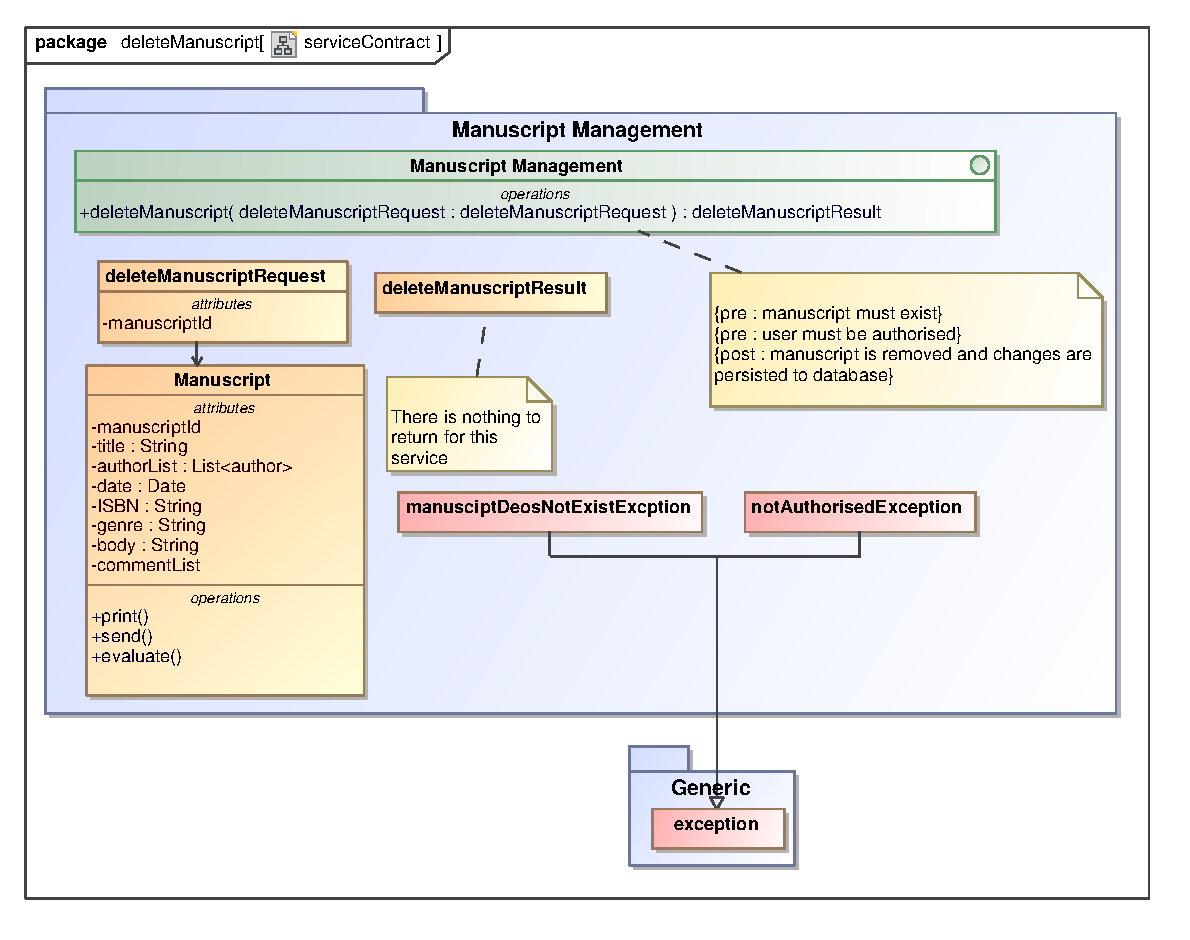
\includegraphics[height=330px, width=500px]{epsImages/ManuscriptManagement/deleteManuscript.eps}
\caption{Service contract for deleting a  project (manuscript)}
\end{figure}

\newpage
\item \textbf{Link To Social Media – priority: important}\\
\par{This use case links a project(manuscript) to a social media of choice if conditions are met and creates an automated post on that social media.}

\textbf{Service Contract:}

\begin{figure}[h]
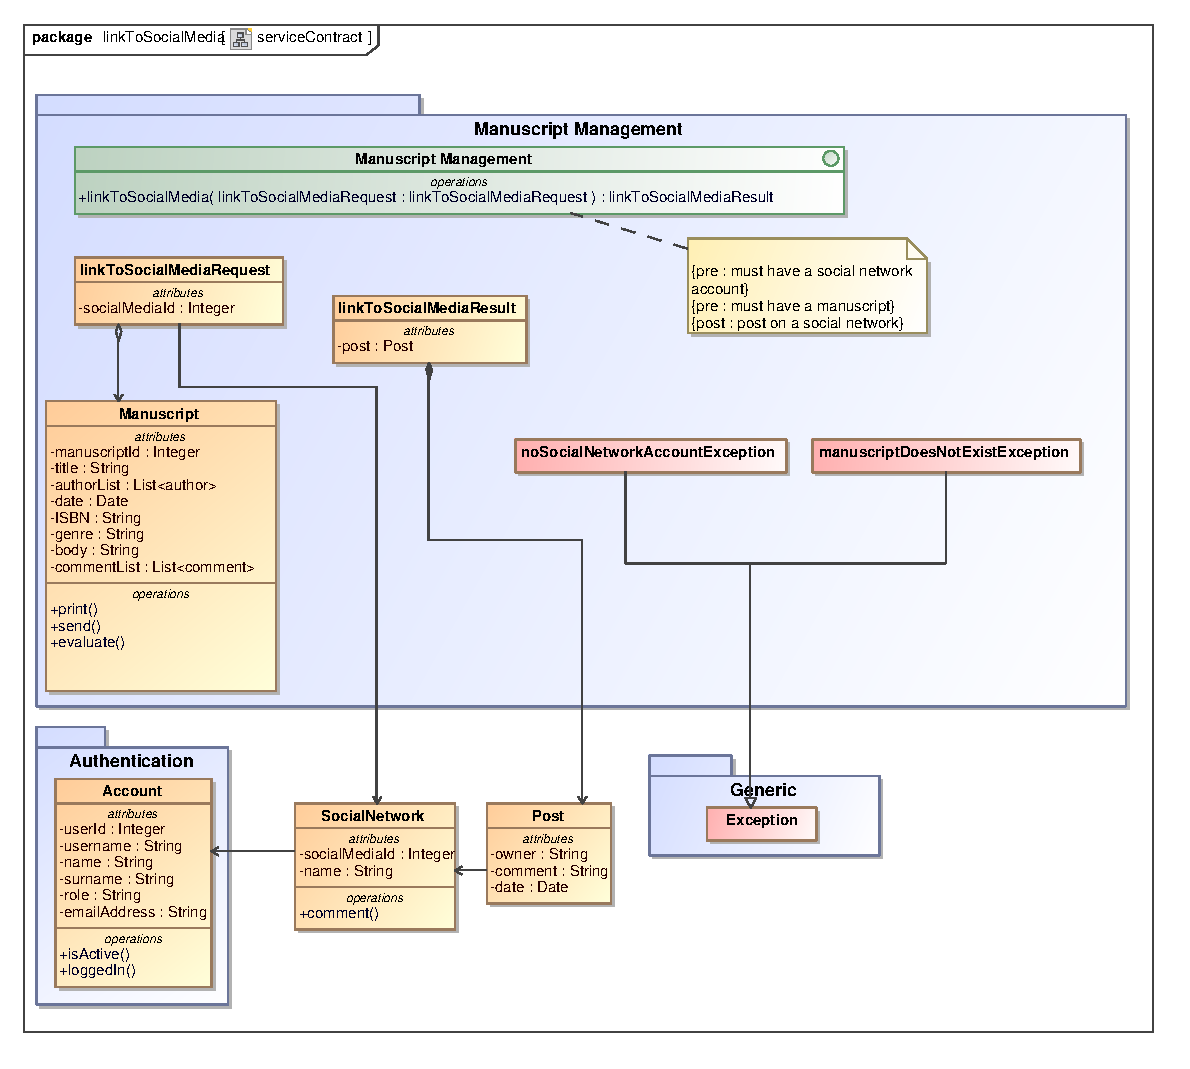
\includegraphics[height=330px, width=500px]{epsImages/ManuscriptManagement/linkToSocialMedia.eps}
\caption{Service contract for linking a  project (manuscript) to a social network}
\end{figure}

\newpage

\item \textbf{Edit Manuscript – priority: critical}
\par{This use case which allows one to edit a manuscript if authorized and afterwards changes are persisted to database.}

\textbf{Service Contract:}

\begin{figure}[h]
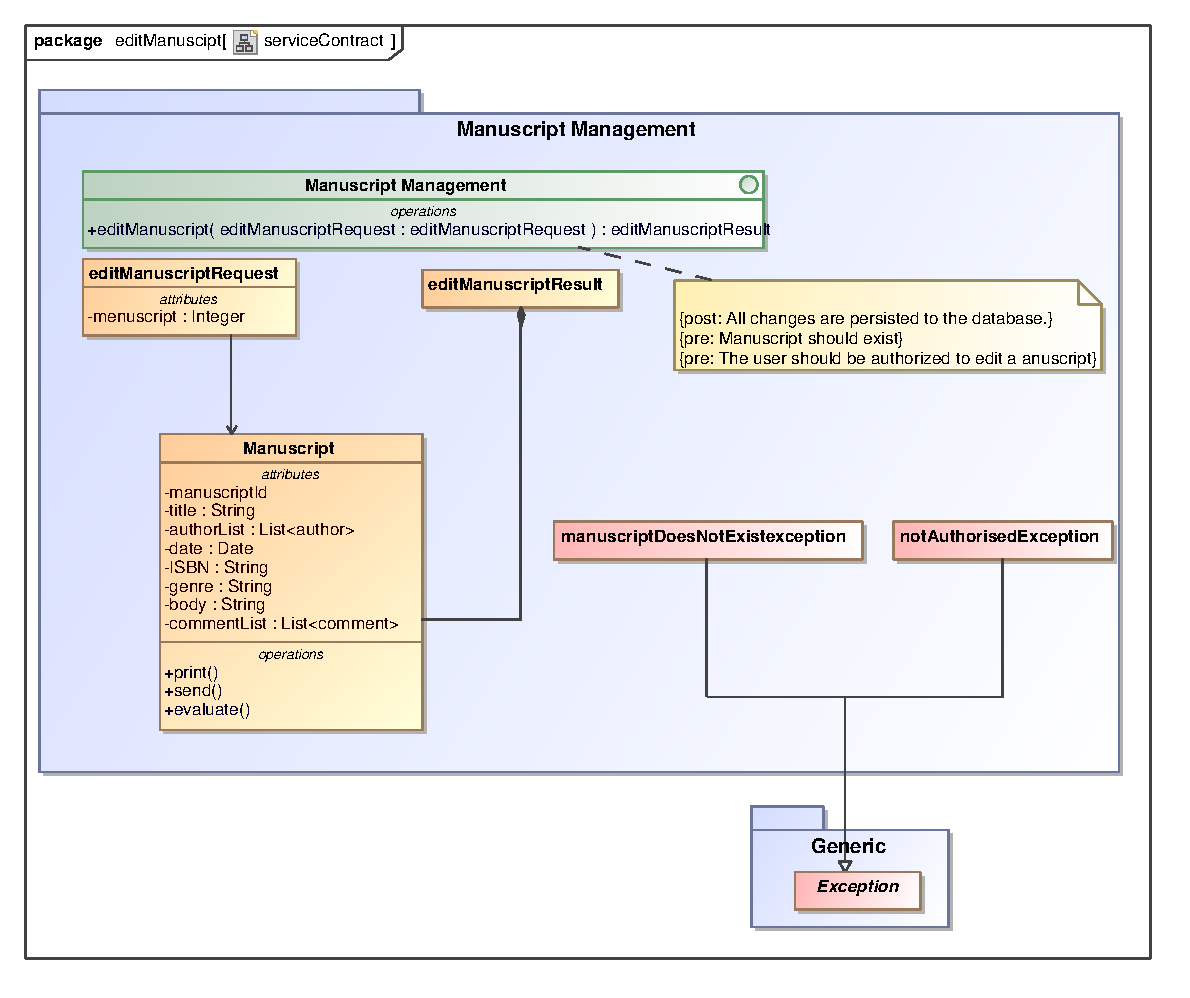
\includegraphics[height=330px, width=500px]{epsImages/ManuscriptManagement/editManuscript.eps}
\caption{Service contract for editing a  project (manuscript)}
\end{figure}
\newpage

\item \textbf{Evaluate Manuscript - priority: critical}
\par{This use case allows an agent or an editorial to evaluate the manuscript and to give the according feedback to the author, such as a comment or editorial letter.}

\textbf{Service Contract:}

\begin{figure}[h]
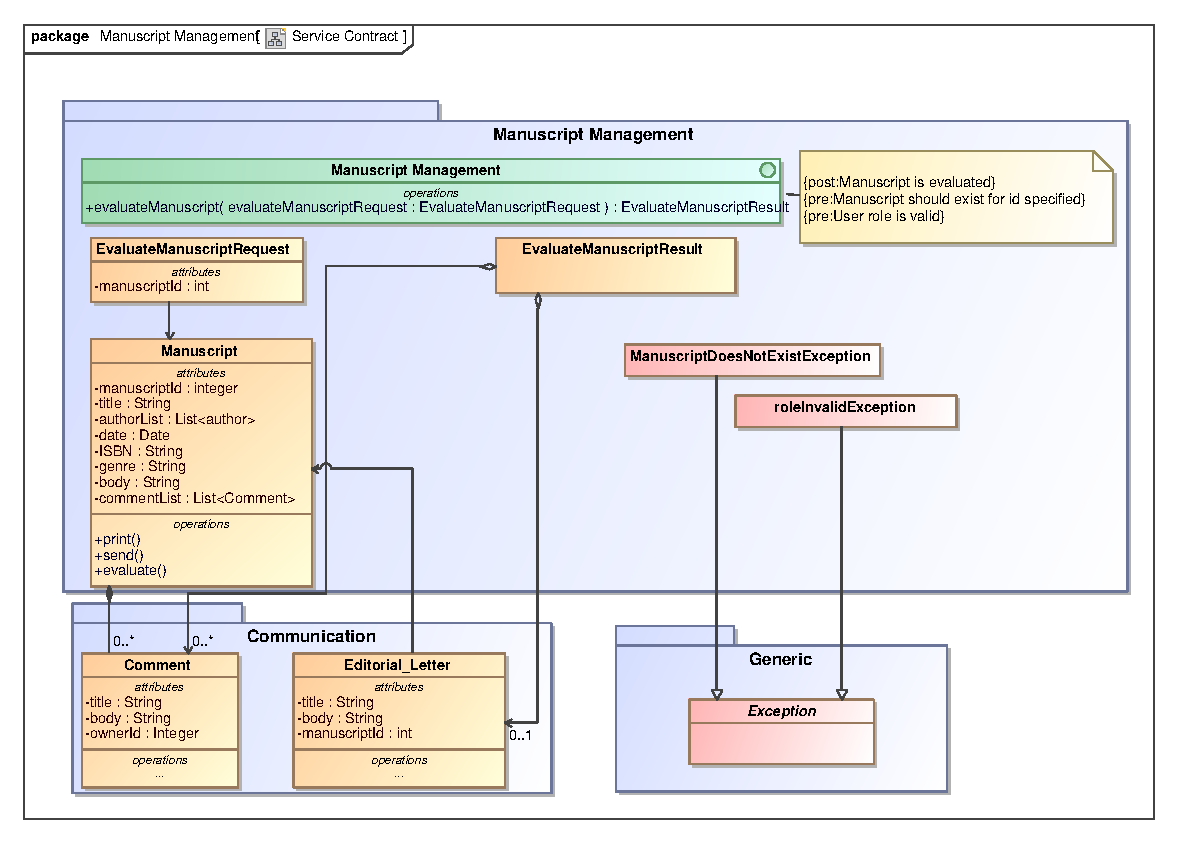
\includegraphics[height=240px, width=500px]{epsImages/ManuscriptManagement/EvaluateManuscript.eps}
\caption{Service contract for evaluating a manuscript}
\end{figure}

\textbf{Process Specification (Activity diagram):}
\begin{figure}[h]
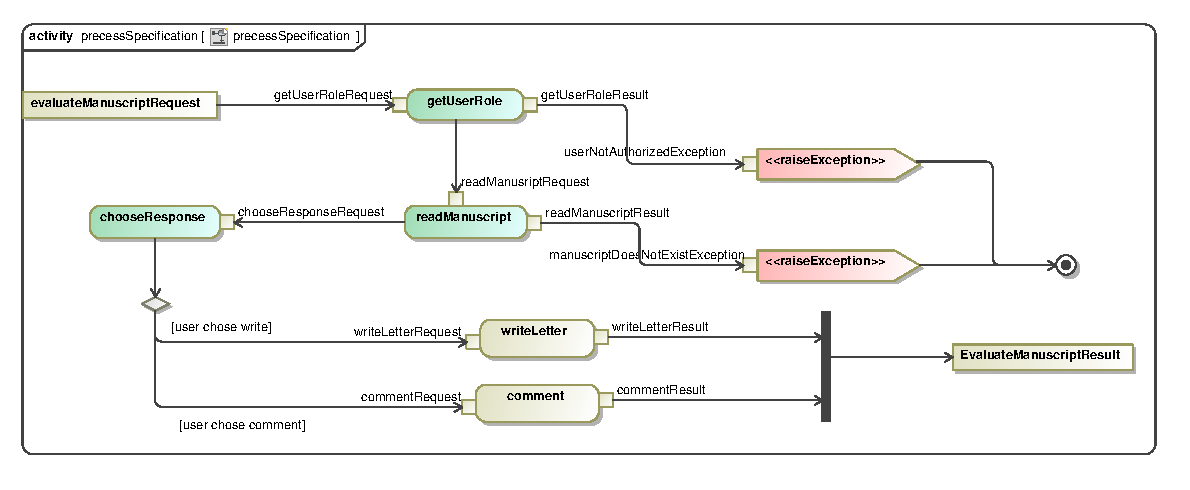
\includegraphics[height=200px, width=500px]{epsImages/ManuscriptManagement/EvaluateActivity.eps}
\caption{Process Specification for evaluating a manuscript}
\end{figure}

\newpage
\item \textbf{Read Manuscript - priority: critical}
\par{The use case grants access to users to view/read a manuscript, under the conditions that the user is authorized and that the manuscript still exists.}

\textbf{Service Contract:}

\begin{figure}[h]
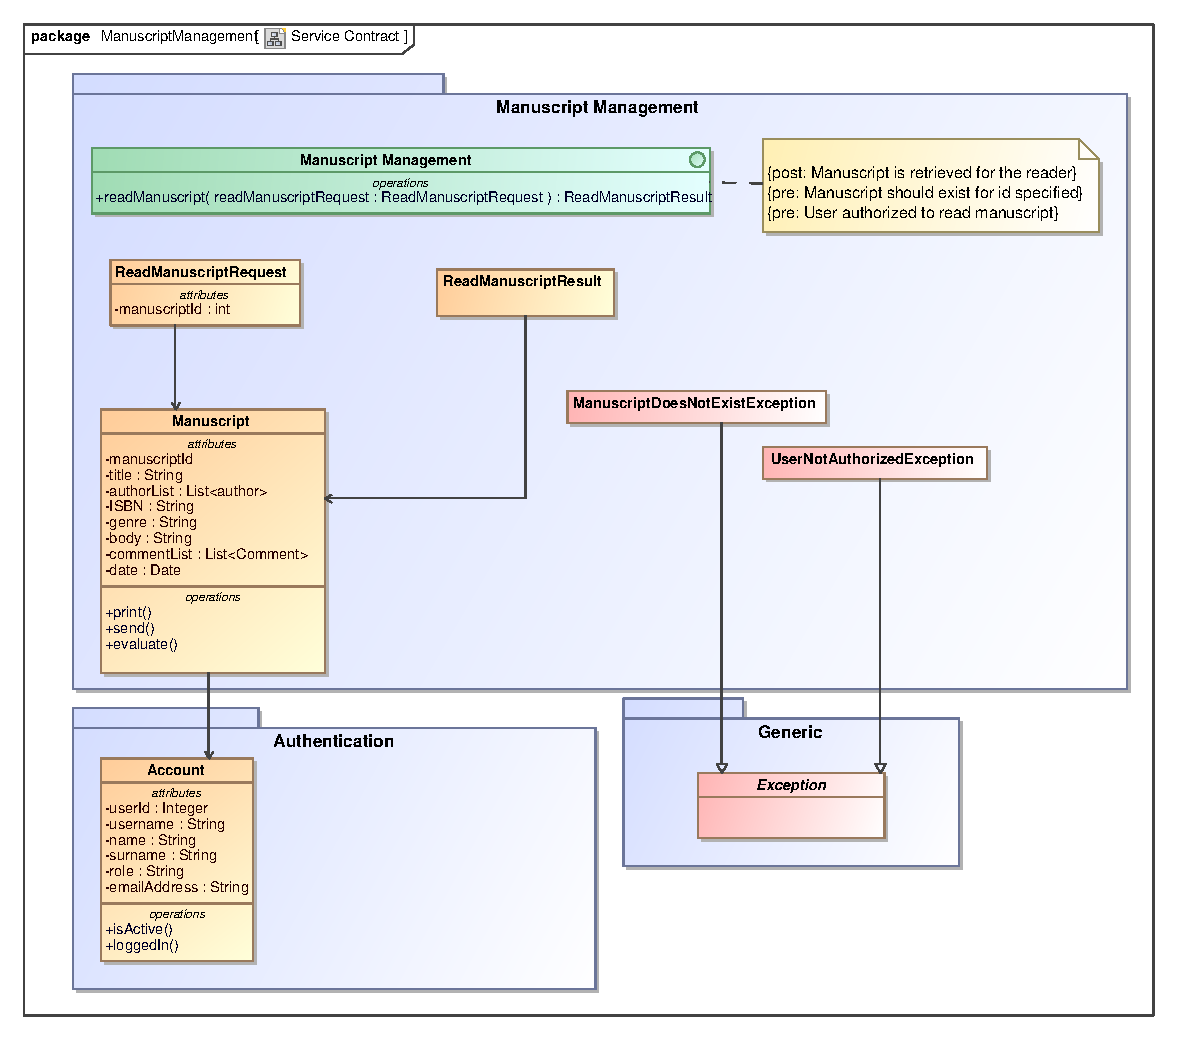
\includegraphics[height=330px, width=500px]{epsImages/ManuscriptManagement/ReadManuscript.eps}
\caption{Service contract for reading a manuscript}
\end{figure}

\newpage
\item \textbf{Send Manuscript - priority: critical}
\par {This use case allows a user link another user on the system to the manuscript. This allows the recipient to access it and, depending on the privileges afforded by the owner of the manuscript, be able to read/modify it.}

\textbf{Service Contract:}

\begin{figure}[h]
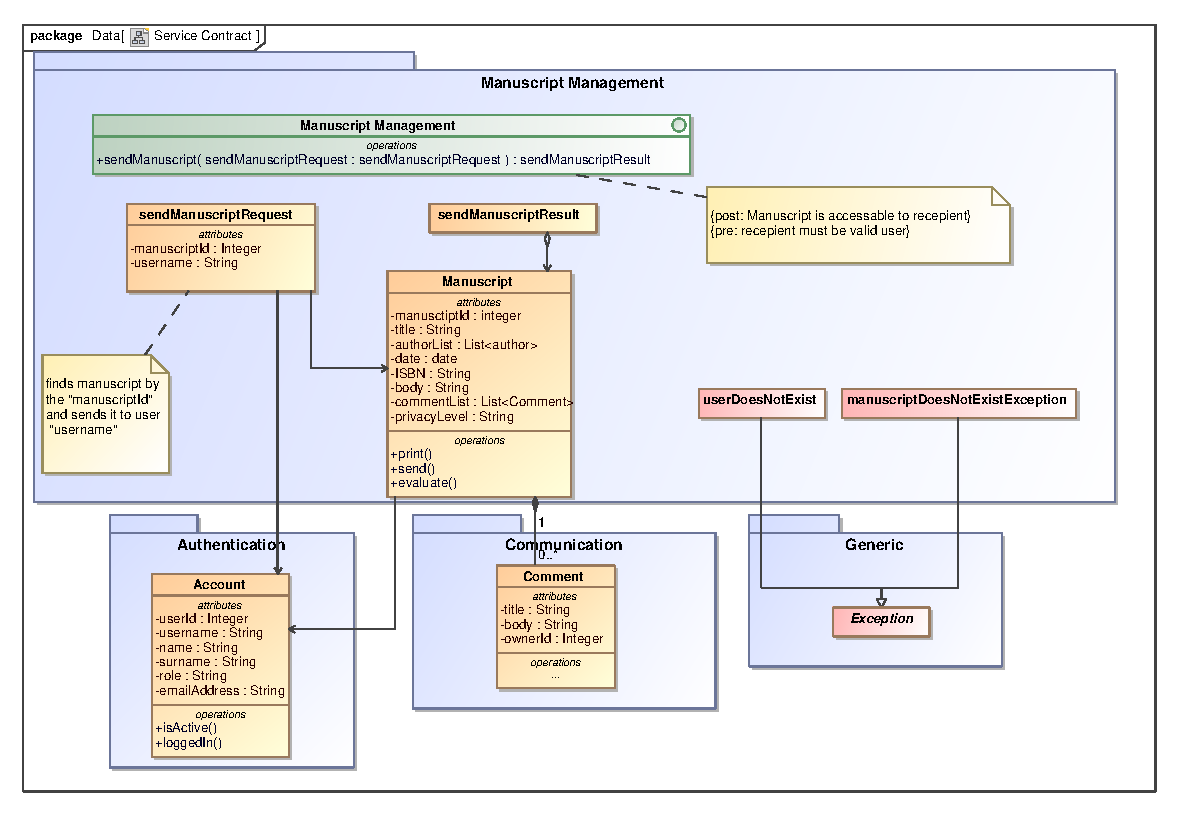
\includegraphics[height=330px, width=500px]{epsImages/ManuscriptManagement/sendManuscriptServiceContract.eps}
\caption{Service contract for sending a manuscript}
\end{figure}
 \newpage
\subsubsection{Domain Model} 
\par {This module will keep a manuscript in the database as well as be connected to all the other modules needed to perform the necessary tasks such as communication, adding authors,editors,agents etc, the modules connected to this module at the current stage of management are: Communication, Authentication as well as the external classes required for linking the manuscript to social media.}

 \begin{figure}[h]
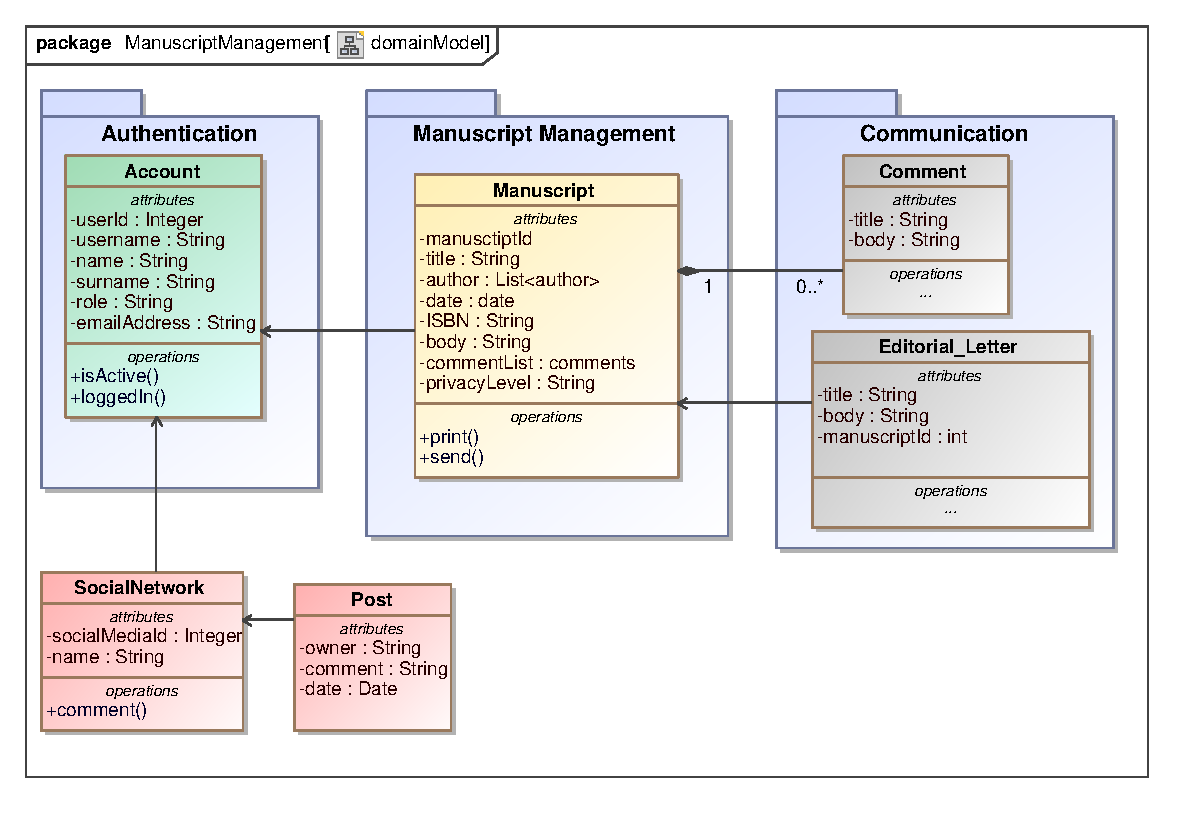
\includegraphics[height=350px, width=500px]{epsImages/DomainModels/ManuscriptManagement.eps}
\caption{Domain model for managing a manuscript}
\end{figure}

\end{enumerate}
